\documentclass[reprint,aps,pra,longbibliography]{revtex4-2}

\usepackage[T1]{fontenc}
\usepackage[utf8]{inputenc}
\usepackage{graphicx}
\usepackage{amsmath,amssymb}
\usepackage{siunitx}
\usepackage{hyperref}
\usepackage{orcidlink}
\usepackage{xcolor}
\usepackage{needspace}
\usepackage{tikz}
\usetikzlibrary{calc,arrows.meta,decorations.pathmorphing,positioning}

\hypersetup{
  colorlinks=true,
  linkcolor=blue,
  citecolor=blue,
  urlcolor=blue
}

\usepackage{pgfplots}
\pgfplotsset{compat=1.18}

\begin{document}

\title{Traction Constraints and the Physics of Faster-Than-the-Wind Travel}

\author{Karl Svozil \orcidlink{0000-0001-6554-2802}}
\affiliation{Institute for Theoretical Physics, TU Wien,
Wiedner Hauptstra{\ss}e 8-10/136, 1040 Vienna, Austria}
\email{karl.svozil@tuwien.ac.at}

\begin{abstract}

Wind-driven vehicles without an auxiliary onboard power source can travel directly downwind faster than the wind. Their drivetrain couples moving air to stationary ground, or to water at rest in the far field, and exchanges momentum between these environments. On land, rolling without slip provides the traction constraint: the ground supplies a tangential force, but its instantaneous contact power is zero in the ground frame. A wheel-driven propeller can nevertheless produce thrust at and above the wind speed. An explicit actuator-disk force and power balance shows how positive shaft power can coexist with a decrease of air kinetic energy in that frame. Gearbox and lever analogies illustrate the associated force--speed tradeoff, while a sliding-boat thought experiment distinguishes internal rearrangement from translation of a closed system's center of mass. The treatment emphasizes reference frames, the limits of ideal constraints, and applications to physics teaching.

\end{abstract}

\maketitle

\section{Introduction: A Counter-Intuitive Phenomenon}

The ability of a wind-powered vehicle to travel directly downwind faster than the wind itself appears paradoxical~\cite{Blackford1978,Stong1975,McDonald2021}. At first glance, such motion seems to violate energy conservation---like pulling oneself up by one's own bootstraps. Yet this is not a theoretical curiosity but an experimentally verified reality. The principle was analyzed as early as 1969 by Bauer~\cite{Bauer1969,bauer1971sailing,bauer1974taking}, and later by Gaunaa et al.~\cite{Gaunaa2009} and McDonald~\cite{McDonald2021} among others~\cite{khan2013analysis,AAPT2013}.


The ``Blackbird'' land yacht~\cite{nahon-2023} reached approximately 2.8 times the true wind speed directly downwind and, in its upwind configuration, 2.1 times the wind speed directly upwind~\cite{nalsa2010}. The phenomenon appeared in the United States Physics Olympiad~\cite{AAPT2013} and became the subject of a public wager documented by Veritasium in June 2021~\cite{Veritasium2021,veritasium_2021_physics}.



The misunderstanding arises from picturing the vehicle as a passive body pushed by the air alone. A conventional sailboat can exceed the true wind speed on a reach, or achieve a downwind velocity made good greater than the wind by sailing at an angle and jibing. Sustained travel \emph{directly} downwind above the wind speed instead requires thrust when the apparent wind vanishes or reverses.

For the vehicles considered here, that thrust is enabled by coupling air to ground or water. Ideal wheel--ground traction imposes rolling without slip and supplies reaction forces without doing work at the contact in the ground frame; hydrodynamic coupling instead entails induced flow and wake losses. We first examine the two operating modes and their force and power balances, then compare watercraft and aircraft in uniform wind. Gearbox, lever, and sliding-boat analogies develop the mechanical intuition. Section~\ref{sec:pedagogy} provides teaching activities and exercises.


\section{The Physics of Faster-Than-the-Wind Travel}


Throughout, ``faster than the wind'' means motion parallel to the true wind, measured in the ground/water frame \(G\). ``Wind-driven'' excludes any auxiliary onboard source supplying net work in sustained operation; start-up transients are treated separately.

\paragraph*{Reference frames and sign conventions.}
In \(G\), the ground and the far-field water are at rest; currents are neglected. Let \(v_w>0\) be the true wind speed and \(v\) the signed vehicle velocity along the wind axis. Positive \(v\) is downwind and negative \(v\) is upwind. In the momentarily comoving vehicle frame \(C\), the far-field apparent-wind component is
\[
v_a=v_w-v.
\]
Thus \(v_a>0\) denotes air approaching from behind, \(v_a=0\) the crossover, and \(v_a<0\) air approaching from ahead. We use \(G\) for vehicle motion and contact work, and \(C\) for local rotor-flow calculations. When the vehicle accelerates, steady actuator-disk formulas in \(C\) are used only as a quasi-steady approximation, neglecting flow-storage and acceleration corrections.

The drivetrain exchanges momentum between air and ground, trading force against speed. In downwind operation the rolling wheels drive the rotor as a \emph{fan}, requiring positive shaft power; in upwind operation the rotor acts as a \emph{turbine} and drives the wheels. Gearing, blade pitch, loading, and losses determine the operating point. The direction of shaft-power transfer must be distinguished from the change of fluid kinetic energy in \(G\), as shown below.



\paragraph*{Relation to Bernoulli's principle.}
In the ideal, locally steady rotor frame, Bernoulli's equation applies separately upstream and downstream of the actuator disk. Across the disk there is a pressure jump: a fan adds mechanical energy to the flow in that frame, whereas a turbine extracts it. This describes the pressure field but must be combined with the drivetrain and vehicle force balances to explain faster-than-the-wind travel.


\subsection{Downwind Faster Than the Wind}

\begin{figure*}[htbp]
\centering
\begin{tabular}{@{}c@{\hspace{6mm}}c@{}}
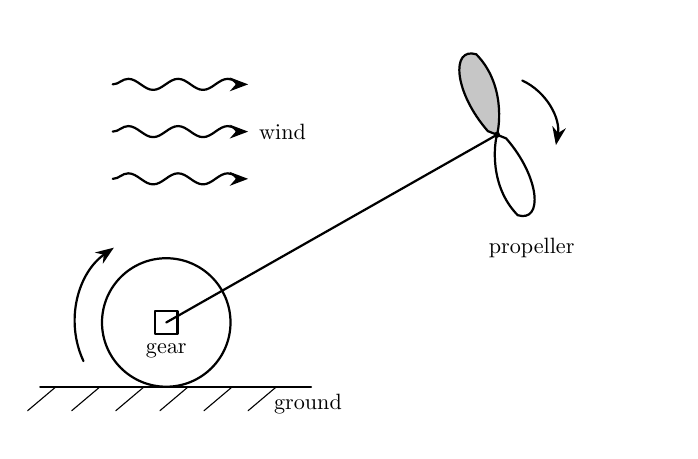
\begin{tikzpicture}[
    scale=0.8, transform shape,
    line cap=round,
    line join=round,
    >=Stealth,
    font=\normalsize
  ]
  \useasboundingbox (-2.2,-0.7) rectangle (8.0,5.7);

  % Key points
  \def\rW{1.02}
  \coordinate (W) at (0,\rW);     % wheel / gear center: tangent to ground
  \coordinate (P) at (5.25,4.00); % propeller center

  % Shaft / blade orientation
  \def\thS{28.5}                   % shaft angle
  \pgfmathsetmacro{\thB}{\thS+180} % blade orientation

  % Ground
  \draw[thick] (-2.0,0) -- (2.3,0);
  \node[below] at (2.25,0) {ground};
  \foreach \x in {-1.75,-1.05,-0.35,0.35,1.05,1.75}{
    \draw (\x,0) -- ++(-0.45,-0.38);
  }

  % Wind arrows: equal length, equal spacing
  \foreach \y in {4.80,4.05,3.30}{
    \draw[->,thick,decorate,decoration={snake,amplitude=2pt,segment length=18pt}]
      (-0.85,\y) -- (1.30,\y);
  }
  % Wind label to the right of the wind block
  \node[anchor=west] at (1.35,4.05) {wind};

  % Wheel / gear
  \draw[thick] (W) circle (\rW);
  \draw[thick] ($(W)+(-0.18,-0.18)$) rectangle ($(W)+(0.18,0.18)$);
  \node at ($(W)+(0,-0.45)$) {gear};

  % Drivetrain / shaft
  \draw[thick] (W) -- (P);

  % Wheel rotation arrow (clockwise for rightward rolling)
  \draw[->,thick] ($(W)+(205:1.45)$)
    arc[start angle=205,end angle=125,radius=1.45];

  % Propeller blades
  % Unshaded blade
  \begin{scope}[shift={(P)}, rotate=\thB]
    \path[draw=black,thick,fill=white]
      (0,0)
      .. controls (0.10,0.10) and (0.50,0.65) .. (0.32,1.28)
      .. controls (0.02,1.58) and (-0.28,0.92) .. (-0.10,0.12)
      -- cycle;
  \end{scope}

  % Shaded blade
  \begin{scope}[shift={(P)}, rotate={\thB+180}]
    \path[draw=black,thick,fill=gray!45]
      (0,0)
      .. controls (0.10,0.10) and (0.50,0.65) .. (0.32,1.28)
      .. controls (0.02,1.58) and (-0.28,0.92) .. (-0.10,0.12)
      -- cycle;
  \end{scope}

  % Propeller hub
  \fill (P) circle (1.4pt);

  % Propeller rotation arrow (clockwise)
  \draw[->,thick] ($(P)+(65:0.95)$)
    arc[start angle=65,end angle=-10,radius=0.95];

  % Propeller label
  \node at ($(P)+(0.55,-1.8)$) {propeller};

\end{tikzpicture}
&
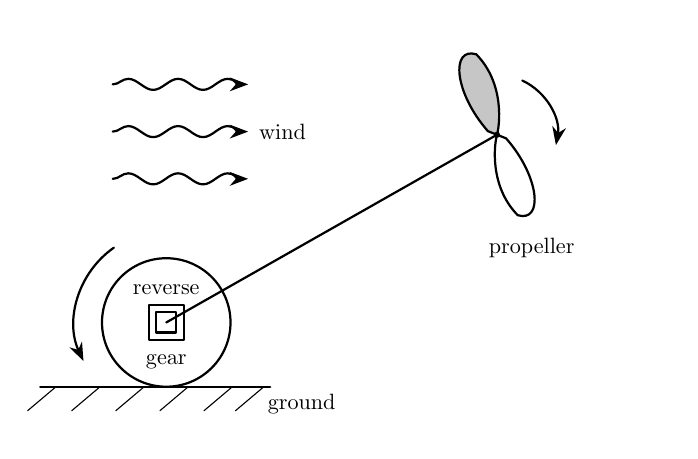
\begin{tikzpicture}[
    scale=0.8, transform shape,
    line cap=round,
    line join=round,
    >=Stealth,
    font=\normalsize
  ]
  \useasboundingbox (-2.2,-0.7) rectangle (8.0,5.7);

  % Key points
  \def\rW{1.02}
  \coordinate (W) at (0,\rW);     % wheel / reverse-gear center: tangent to ground
  \coordinate (P) at (5.25,4.00); % propeller center

  % Shaft / blade orientation
  \def\thS{28.5}                   % shaft angle
  \pgfmathsetmacro{\thB}{\thS+180} % same blade orientation as the downwind panel

  % Ground
  \draw[thick] (-2.0,0) -- (1.65,0);
  \node[below] at (2.15,0) {ground};
  \foreach \x in {-1.75,-1.05,-0.35,0.35,1.05,1.55}{
    \draw (\x,0) -- ++(-0.45,-0.38);
  }

  % Wind arrows: equal length, equal spacing
  \foreach \y in {4.80,4.05,3.30}{
    \draw[->,thick,decorate,decoration={snake,amplitude=2pt,segment length=18pt}]
      (-0.85,\y) -- (1.30,\y);
  }
  % Wind label to the right of the wind block
  \node[anchor=west] at (1.35,4.05) {wind};

  % Wheel / reverse gear
  \draw[thick] (W) circle (\rW);
  \draw[thick] ($(W)+(-0.28,-0.28)$) rectangle ($(W)+(0.28,0.28)$);
  \draw[thick] ($(W)+(-0.16,-0.16)$) rectangle ($(W)+(0.16,0.16)$);
  \node[align=center] at ($(W)+(0,+0.52)$) {reverse};
  \node[align=center] at ($(W)+(0,-0.62)$) {gear};

  % Drivetrain / shaft
  \draw[thick] (W) -- (P);

  % Wheel rotation arrow (counterclockwise, opposite to downwind)
  \draw[->,thick] ($(W)+(125:1.45)$)
    arc[start angle=125,end angle=205,radius=1.45];

  % Propeller blades
  % Unshaded blade
  \begin{scope}[shift={(P)}, rotate=\thB]
    \path[draw=black,thick,fill=white]
      (0,0)
      .. controls (0.10,0.10) and (0.50,0.65) .. (0.32,1.28)
      .. controls (0.02,1.58) and (-0.28,0.92) .. (-0.10,0.12)
      -- cycle;
  \end{scope}

  % Shaded blade
  \begin{scope}[shift={(P)}, rotate={\thB+180}]
    \path[draw=black,thick,fill=gray!45]
      (0,0)
      .. controls (0.10,0.10) and (0.50,0.65) .. (0.32,1.28)
      .. controls (0.02,1.58) and (-0.28,0.92) .. (-0.10,0.12)
      -- cycle;
  \end{scope}

  % Propeller hub
  \fill (P) circle (1.4pt);

  % Propeller rotation arrow (clockwise)
  \draw[->,thick] ($(P)+(65:0.95)$)
    arc[start angle=65,end angle=-10,radius=0.95];

  % Propeller label
  \node at ($(P)+(0.55,-1.8)$) {propeller};

\end{tikzpicture}
\\
(a) Downwind Operation & (b) Upwind Operation
\end{tabular}
\caption{Schematic of a wind-driven vehicle's operation.  Arrows indicate the direction of rotation. The pitch of the propeller blades is indicated by the darker shade of the blade facing the rear.
(a) For downwind travel faster than the wind, the wheels drive the propeller, which pushes air backward to generate thrust.
(b) For upwind travel, the wind turns the propeller (acting as a turbine), which drives the wheels, whose traction propels the vehicle against the wind.}
\label{fig:vehicle_operation}
\end{figure*}


Consider the cart in Fig.~\ref{fig:vehicle_operation}(a). A tailwind can initiate its motion; as it rolls, the wheel-linked propeller pushes air rearward relative to the cart. Near \(v=v_w\), the far-field apparent wind tends to zero, but the driven propeller induces its own flow. Above the crossover, it continues to operate as a fan in the approaching headwind. Figure~\ref{fig:dimensionless_plots}(b) shows this reversal of \(v_a\).

The achievable speed depends on rotor performance, transmission losses, body drag, rolling resistance, and available traction. The rigid-rack analogies developed later establish the mechanical possibility but do not prescribe the operating speed of a real propeller cart.

\subsubsection{Explicit force and power balance}
\label{sec:downwind-power}

Consider \(v\geq v_w>0\). Let \(T>0\) be the forward propeller thrust, \(R>0\) the magnitude of the retarding wheel--ground traction force, and \(m_c\) the cart mass. Neglect body drag, mechanical losses, and changes of rotational kinetic energy. The latter approximation retains translational acceleration while neglecting the additional power needed to accelerate the rotating components.

In the quasi-steady frame \(C\), the upstream air approaches the propeller with speed \(U=v-v_w\). For an ideal actuator disk of area \(A\), let \(u_i>0\) be the induced speed at the disk. Assume incompressible axial flow, negligible swirl, and equal ambient static pressure in the far upstream and downstream regions. The downstream speed is \(U+2u_i\), and
\begin{align}
\dot m &= \rho A(U+u_i), & T&=2\dot m\,u_i,
\label{eq:cart-mass-thrust}\\
P_{\rm shaft}
 &=\tfrac12\dot m\bigl[(U+2u_i)^2-U^2\bigr]\nonumber\\
 &=T(U+u_i)=T(v-v_w+u_i).
\label{eq:cart-shaft-power}
\end{align}
This positive shaft power is supplied by the wheels. Their retarding traction changes translational energy at the rate \(-Rv\), while the corresponding torque transfers \(+Rv\) to the drivetrain. These contributions cancel at the ideal rolling contact, whose actual power in \(G\) is zero. Under the stated assumptions,
\begin{equation}
Rv=P_{\rm shaft}.
\label{eq:cart-wheel-power}
\end{equation}
The vehicle force balance is therefore
\begin{align}
m_c\dot v&=F_{\rm drive}=T-R\nonumber\\
 &=\frac{T}{v}(v_w-u_i).
\label{eq:cart-net-drive}
\end{align}
At the crossover \(v=v_w\), the propeller still processes the induced mass flow \(\rho A u_i\) and consumes power \(Tu_i\). Positive thrust and positive acceleration coexist when \(u_i<v_w\); neither follows merely from the vanishing far-field apparent wind.

The energy source becomes explicit on returning to \(G\). The far-upstream and far-downstream air velocities are \(v_w\) and \(v_w-2u_i\). Thus the net air kinetic-energy flux change is
\begin{align}
\Delta\dot E_{\rm air,G}
 &=\tfrac12\dot m\bigl[(v_w-2u_i)^2-v_w^2\bigr]\nonumber\\
 &=P_{\rm shaft}-Tv=-T(v_w-u_i).
\label{eq:cart-air-power}
\end{align}
Meanwhile \(\dot K_{\rm cart}=F_{\rm drive}v=T(v_w-u_i)\). The cart's gain equals the air's loss. Positive fan shaft power therefore does not imply that the air gains kinetic energy in the ground frame~\cite{Gaunaa2009,AAPT2013}.

For a drivetrain efficiency \(0<\eta\leq1\), while retaining the ideal rotor model, \(P_{\rm shaft}=\eta Rv\). If \(D\geq0\) denotes additional retarding forces, the available force becomes
\begin{equation}
F_{\rm drive}=T-\frac{P_{\rm shaft}}{\eta v}-D.
\label{eq:cart-losses}
\end{equation}
Rotor losses and rotational acceleration require further shaft power. These effects and traction limits reduce the achievable speed and must be included in a detailed performance model.


\subsection{Upwind Travel}


In Fig.~\ref{fig:vehicle_operation}(b), the rotor operates as a turbine and transmits shaft power to the wheels, which propel the vehicle upwind. Its aerodynamic force is downwind, so the upwind wheel traction must exceed that force and the other resistances. As in downwind operation, ideal ground contact supplies momentum exchange while doing no contact work in \(G\).


\section{Why Not in the Air?}
\label{wind:whynotintheair}


A free-flying aircraft in steady, spatially uniform wind, without an auxiliary energy source, cannot use this particular air--ground drivetrain mechanism. A conventional powered fixed-wing aircraft with an airspeed of \SI{500}{km/h} in a \SI{100}{km/h} tailwind has a ground speed of \SI{600}{km/h}; that example does not demonstrate propulsion powered solely by the uniform wind. At zero airspeed, a conventional fixed wing cannot supply its usual aerodynamic lift.

The restriction is to uniform wind and this coupling mechanism. Wind shear provides air regions with different velocities and can offer another energy source; it lies outside the present model. More generally, the two interacting environments need not be different substances: two regions of the same medium in relative motion can serve the corresponding roles~\cite{Gaunaa2009}.


\Needspace{8\baselineskip}
\section{On Water: Fluid-Mediated Constraints, Slip, and Two Propulsion Scenarios}
\label{sec:water-sail-prop}


Watercraft couple air and water, but their water-side reaction is mediated by fluid motion rather than a rigid rolling constraint. Induced velocities and wakes incur an energy cost. In \(G\), the far-field water is at rest; locally, the hull, foils, and propulsors disturb it. The axial velocities retain the convention \(v_a=v_w-v\), illustrated in Fig.~\ref{fig:water-frame}. Local rotor formulas below use the quasi-steady vehicle frame \(C\).


\begin{figure}[tb]
\centering
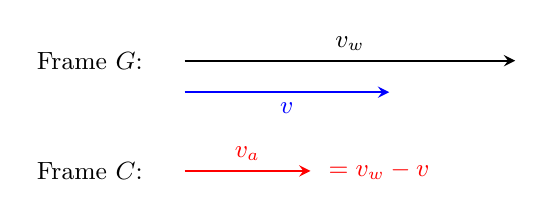
\begin{tikzpicture}[>=stealth, font=\small, thick]

% --- Frame G ---
\node[anchor=east] at (-0.4,0.8) {Frame \(G\):};
\draw[->] (0,0.8) -- (4.2,0.8) node[midway, above] {\(v_w\)};
\draw[->, blue] (0,0.4) -- (2.6,0.4) node[midway, below] {\(v\)};

% --- Frame C ---
\node[anchor=east] at (-0.4,-0.6) {Frame \(C\):};
\draw[->, red] (0,-0.6) -- (1.6,-0.6) node[midway, above] {\(v_a\)};
\node[right, red] at (1.7,-0.6) {\(= v_w - v\)};

\end{tikzpicture}
\caption{Minimal kinematic definitions for Sec.~\ref{sec:water-sail-prop}. In the laboratory frame \(G\), the true wind is \(v_w\) and the boat speed is \(v\). In the vehicle frame \(C\), the apparent-wind velocity is \(v_a = v_w - v\). Vectors are aligned at a common origin; for \(v > v_w\), the apparent-wind velocity \(v_a\) reverses direction.}
\label{fig:water-frame}
\end{figure}

\subsection{Scenario 1: Geometric coupling (sails and keels/foils)}


A conventional sailboat couples aerodynamic and hydrodynamic forces: the sail produces a force generally dominated by lift relative to the apparent airflow, while the keel or foils provide sideforce that limits lateral drift. For tacking and reaching, the apparent wind is a vector rather than the axial scalar \(v_a\) used in the one-dimensional examples.


\paragraph*{Against the wind (upwind progress):}
A sailboat does not go straight into the wind; it makes upwind progress by
tacking.  The keel/foil must operate at a finite angle of attack to generate
sideforce, so some leeway and an associated induced-drag penalty are unavoidable
in practice.  Unlike ideal rolling contact, the water-side reaction cannot be
treated as a kinematic constraint that transmits arbitrary lateral force at
zero power cost: generating sideforce requires exchanging momentum with the
water and typically leaves kinetic energy in the wake.

\paragraph*{With the wind (downwind):}
It is common for fast craft (skiffs, catamarans, iceboats) to achieve a downwind
\emph{velocity made good}---the component of velocity directed toward the downwind destination---that exceeds the true wind speed by sailing at
an angle (broad reaching) and jibing; in that regime the apparent wind tends to
increase and rotate forward, keeping the sail in a lifting condition.

By contrast, a conventional sailboat generally cannot sustain a speed exceeding
the wind \emph{directly dead downwind}.  If $v \parallel v_w$
and $v \to v_w$, then $v_a \to 0$ and a passive sail loses
the aerodynamic drive needed to overcome water drag.  To exceed the wind speed
\emph{directly} downwind requires a mechanism that can continue to produce thrust
even when the apparent wind vanishes or reverses---that is, an explicit
``mechanical transformer'' rather than a purely geometric sail--keel coupling.

\subsection{Scenario 2: Mechanical coupling (coupled air and water propellers/turbines)}

To reproduce the Blackbird-style ``two-media gearbox'' on water, one may couple an air turbine or propeller to a water turbine or propeller via a shaft and, if desired, gearing. Stong's 1975 column reports Seelye Martin's description of the ``push--me--pull--you'' toy boat, credited to Peter Kauffman and Eric Lindahl~\cite{Stong1975}.


For the local calculation, work in \(C\) and assume steady incompressible flow through the propulsor, negligible swirl, and equal far-field static pressures. If \(u_{\rm in,C}\) and \(u_{\rm out,C}\) are signed axial velocities and \(\dot m\) is the mass flow rate, momentum and energy transfer give
\begin{align}
F_{\rm fluid}&=\dot m(u_{\rm out,C}-u_{\rm in,C}),
\label{eq:fluid-force}\\
P_{\rm shaft}&=\tfrac12\dot m(u_{\rm out,C}^2-u_{\rm in,C}^2).
\label{eq:fluid-shaft-power}
\end{align}
The device experiences the opposite force. Transforming the kinetic-energy flux to \(G\) gives
\begin{equation}
\Delta\dot E_{\rm fluid,G}=P_{\rm shaft}+vF_{\rm fluid},
\label{eq:fluid-frame-power}
\end{equation}
which explains why shaft power and ground-frame fluid energy transfer must be distinguished; Eq.~\eqref{eq:cart-air-power} is the downwind example.

For a fan, let \(U\geq0\) be the upstream speed along the flow, \(\Delta u>0\) the far-wake speed increment, and \(A\) the disk area. With \(T\) denoting the thrust magnitude,
\begin{align}
\dot m&=\rho A\left(U+\frac{\Delta u}{2}\right),
\label{eq:fluid-mass-flow}\\
T&=\dot m\,\Delta u,\qquad
P_{\rm shaft}=T\left(U+\frac{\Delta u}{2}\right).
\label{eq:fluid-disk-power}
\end{align}
For \(\Delta u\ll U\), \(T\approx P_{\rm shaft}/U\): a slowly moving stream can provide a larger force per unit shaft power. This lightly loaded approximation is not valid at \(U=0\), where induced flow still requires finite power. A turbine instead reduces the speed along the stream and extracts shaft power within its applicable momentum-theory regime.

For upwind travel, the air approaches faster than the water in \(C\). An air turbine can therefore drive a water propeller that produces a larger opposing thrust, provided losses are sufficiently small. Downwind above the wind speed, the relative water speed \(v\) exceeds the relative air speed \(v-v_w\): a water turbine can drive an air fan. These roles reproduce the land-vehicle power transfer, with additional water-side wake losses.

The quantitative outcome depends on swept areas, loading, and efficiencies. Since air is much less dense than water, the air rotor generally requires a larger area. A compact, heavily loaded water propulsor produces greater slip and wake losses, while an undersized air rotor may not provide the necessary power. Component sizing and net force balance, rather than stream speed alone, determine whether faster-than-the-wind travel is attainable.


\subsection{The penalty of slip}


Ideal rolling contact exchanges momentum without leaving a moving wake in the ground. A finite water propulsor or lifting foil, by contrast, transfers momentum to water and leaves induced flow and wake energy. Waterborne devices therefore face an additional efficiency penalty, together with hull drag, although the coupling principle is the same. No rigid no-slip relation fixes their speed relative to either fluid.


\section{Building Intuition: Mechanical Analogies}

To deepen this understanding, we employ a series of mechanical analogies that
illustrate velocity amplification, energy transfer between coupled media, and
the role of the external reaction constraint introduced above.

\subsection{The Gearbox Analogy}


The rack-and-gear demonstration of Ref.~\cite{veritasium_2021_physics} isolates velocity amplification and its force tradeoff. Unlike fluid coupling, both rack contacts impose rigid no-slip conditions. Consequently, the resulting exact speed ratios belong to this mechanical model and do not by themselves predict a real cart's speed.

The upper rack represents wind moving at \(v_w\) in \(G\), and the lower rack represents stationary ground. Their common gearbox casing translates at \(v\). The free gear of radius \(r_1\) meshes with a pinion of radius \(r_2\), rigidly attached to the ground-contact gear of radius \(r_3\). The two larger gears are understood to occupy different axial planes, so only the intended pinion mesh occurs.

\subsubsection{Positive Transmission (Downwind)}

In the momentarily comoving frame \(C\), the upper rack has velocity \(v_a=v_w-v\) and the lower rack has velocity \(-v\). Figure~\ref{fig:gearboxes}(a) shows the configuration in \(G\).


\begin{figure*}[htbp]
\centering
\begin{tabular}{@{}c@{\hspace{6mm}}c@{}}
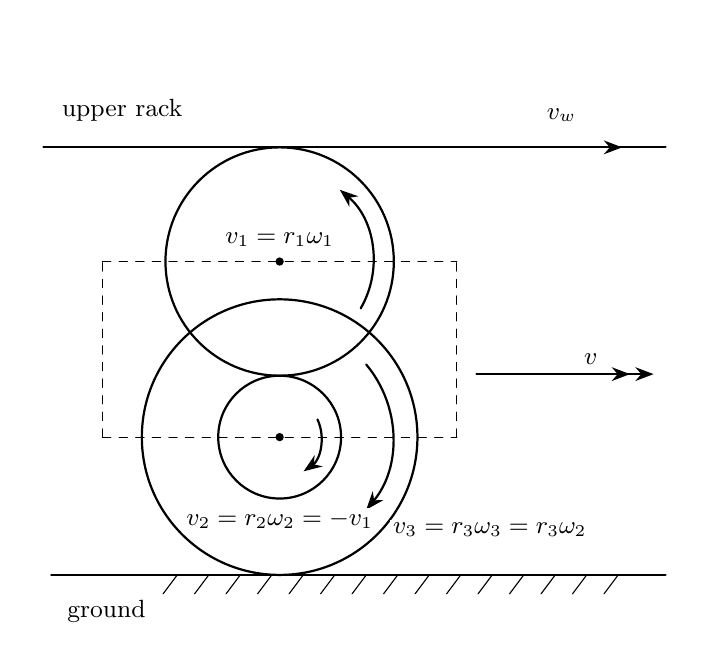
\begin{tikzpicture}[line cap=round,line join=round,>=Stealth,font=\small]
  \useasboundingbox (-3.2,-0.55) rectangle (5.2,6.95);

  % Radii
  \def\rA{1.45}   % upper gear radius r1
  \def\rB{1.75}   % lower gear radius r3
  \def\rP{0.78}   % pinion radius r2
  \def\rI{0.55}   % idler radius (unused here, only for matched sizing)

  % Arrow radii
  \pgfmathsetmacro{\rAa}{0.82*\rA}
  \pgfmathsetmacro{\rBb}{0.82*\rB}
  \pgfmathsetmacro{\rPp}{0.68*\rP}

  % Vertical coordinates
  \pgfmathsetmacro{\yOthree}{\rB}             % lower gear / pinion center
  \pgfmathsetmacro{\yOone}{\rB+\rP+\rA}       % upper gear center (touches pinion)
  \pgfmathsetmacro{\yTop}{\rB+\rP+2*\rA}      % upper rack height

  % Centers
  \coordinate (O3) at (0,\yOthree);
  \coordinate (O1) at (0,\yOone);

  % Upper rack
  \draw[thick] (-3.0,\yTop) -- (4.9,\yTop);
  \node[above] at (-2,\yTop+0.2) {upper rack};
  \draw[->,thick] (2.8,\yTop) -- (4.35,\yTop);
  \node[above] at (3.58,\yTop+0.2) {$v_w$};

  % Dashed box / centerlines
  \draw[dashed] (-2.25,\yOone) -- (2.25,\yOone);
  \draw[dashed] (-2.25,\yOthree) -- (2.25,\yOthree);
  \draw[dashed] (-2.25,\yOthree) -- (-2.25,\yOone);
  \draw[dashed] (2.25,\yOthree) -- (2.25,\yOone);

  % Upper gear
  \draw[thick] (O1) circle (\rA);
  \fill (O1) circle (1.5pt);

  % Lower gear and pinion
  \draw[thick] (O3) circle (\rB);
  \draw[thick] (O3) circle (\rP);
  \fill (O3) circle (1.5pt);

  % Rotation arrows
  % upper gear CCW
 \draw[->,thick] ($(O1)+(-30:\rAa)$)
  arc[start angle=-30,end angle=50,radius=\rAa];
  % lower gear / pinion CW
  \draw[->,thick] ($(O3)+(40:\rBb)$)
    arc[start angle=40,end angle=-40,radius=\rBb];
  \draw[->,thick] ($(O3)+(25:\rPp)$)
    arc[start angle=25,end angle=-55,radius=\rPp];

  % Labels
  \node[fill=white,inner sep=1pt] at (0,\yOone+0.28) {$v_1=r_1\omega_1$};
  \node[fill=white,inner sep=1pt] at (0,\yOthree-1.05) {$v_2=r_2\omega_2=-v_1$};
  \node[below right,fill=white,inner sep=1pt] at (1.4,0.7) {$v_3=r_3\omega_3=r_3\omega_2$};

  % Ground
  \draw[thick] (-2.9,0) -- (4.9,0);
  \node[below] at (-2.2,-0.2) {ground};
  \foreach \x in {-1.3,-0.9,...,4.7}
    \draw (\x,0) -- ++(-0.18,-0.24);

  % vf arrow to the right
  \draw[->,thick] (2.5,2.55) -- (4.45,2.55);
  \draw[->,thick] (3.5,2.55) -- (4.75,2.55);
  \node[above] at (3.95,2.55) {$v$};
\end{tikzpicture}
&
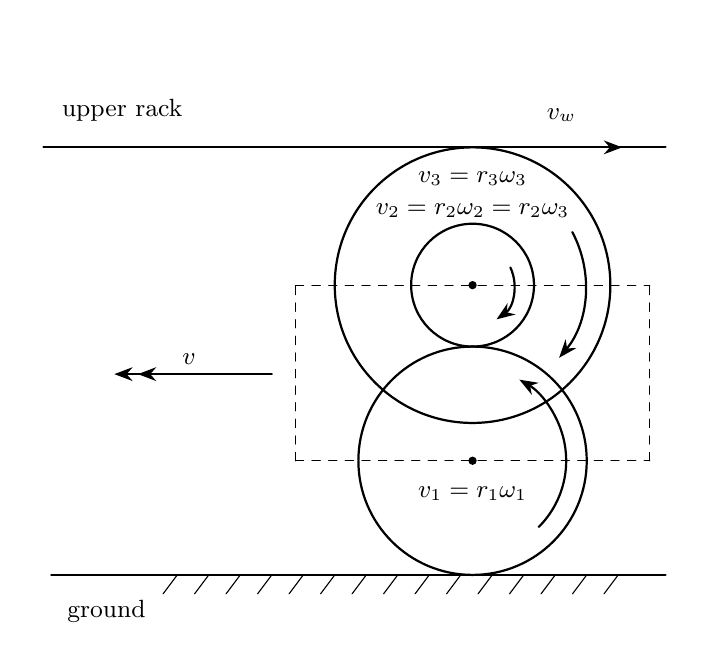
\begin{tikzpicture}[line cap=round,line join=round,>=Stealth,font=\small]
  \useasboundingbox (-3.2,-0.55) rectangle (5.2,6.95);

  % Radii
  \def\rA{1.45}   % lower free gear radius r1
  \def\rB{1.75}   % upper gear radius r3
  \def\rP{0.78}   % pinion radius r2

  % Arrow radii
  \pgfmathsetmacro{\rAa}{0.82*\rA}
  \pgfmathsetmacro{\rBb}{0.82*\rB}
  \pgfmathsetmacro{\rPp}{0.68*\rP}

  % Vertical coordinates for the top--bottom inverted gearbox
  % Lower free gear r1 touches the ground.
  % Pinion r2 and gear r3 share the upper shaft.
  \pgfmathsetmacro{\yOone}{\rA}                  % lower free gear center
  \pgfmathsetmacro{\yOthree}{2*\rA+\rP}          % upper shaft: r3 gear and r2 pinion
  \pgfmathsetmacro{\yTop}{\yOthree+\rB}          % upper rack height


    % Upper rack
    \draw[thick] (-3.0,\yTop) -- (4.9,\yTop);
    \node[above] at (-2,\yTop+0.2) {upper rack};
    \draw[->,thick] (2.8,\yTop) -- (4.35,\yTop);
    \node[above] at (3.58,\yTop+0.2) {$v_w$};


  % Shift the whole geartrain slightly to the RIGHT
  \begin{scope}[xshift=2.45cm]

    % Centers
    \coordinate (O1) at (0,\yOone);
    \coordinate (O3) at (0,\yOthree);

    % Dashed box / centerlines
    \draw[dashed] (-2.25,\yOone) -- (2.25,\yOone);
    \draw[dashed] (-2.25,\yOthree) -- (2.25,\yOthree);
    \draw[dashed] (-2.25,\yOone) -- (-2.25,\yOthree);
    \draw[dashed] (2.25,\yOone) -- (2.25,\yOthree);

    % Upper gear and pinion on common shaft
    \draw[thick] (O3) circle (\rB);
    \draw[thick] (O3) circle (\rP);
    \fill (O3) circle (1.5pt);

    % Lower free gear
    \draw[thick] (O1) circle (\rA);
    \fill (O1) circle (1.5pt);

    % Rotation arrows for upwind solution with r3>r2:
    % upper gear / pinion rotate clockwise; lower gear rotates counter-clockwise.
    \draw[->,thick] ($(O3)+(28:\rBb)$)
  arc[start angle=28,end angle=-40,radius=\rBb];
    \draw[->,thick] ($(O3)+(25:\rPp)$)
      arc[start angle=25,end angle=-55,radius=\rPp];
 \draw[->,thick] ($(O1)+(-45:\rAa)$)
  arc[start angle=-45,end angle=60,radius=\rAa];

    % Labels
    \node[fill=white,inner sep=1pt] at (0,\yOthree+1.35) {$v_3=r_3\omega_3$};
    \node[fill=white,inner sep=1pt] at (0,\yOthree+0.95) {$v_2=r_2\omega_2=r_2\omega_3$};
    \node[fill=white,inner sep=1pt] at (0,\yOone-0.42) {$v_1=r_1\omega_1$};

  \end{scope}

    % Ground
    \draw[thick] (-2.9,0) -- (4.9,0);
    \node[below] at (-2.2,-0.2) {ground};
    \foreach \x in {-1.3,-0.9,...,4.7}
      \draw (\x,0) -- ++(-0.18,-0.24);

  % v arrow stays where it is now
  \draw[->,thick] (-0.15,2.55) -- (-2.10,2.55);
  \draw[->,thick] (-0.10,2.55) -- (-1.80,2.55);
  \node[above] at (-1.15,2.55) {$v$};

\end{tikzpicture}
\\[3mm]
(a) Positive Transmission & (b) Negative Transmission
\end{tabular}
\caption{Rack-and-gear model in \(G\), with upper rack velocity \(v_w\), stationary lower rack, and casing velocity \(v\). Curved arrows show rotation; \(v_k=r_k\omega_k\) are signed circumferential quantities. Actual tooth velocities include casing translation. (a) The free upper gear drives pinion \(r_2\) and ground-contact gear \(r_3\), giving \(v/v_w=r_3/(r_3-r_2)\). (b) Inverting the assembly gives \(v/v_w=-r_2/(r_3-r_2)\). It travels upwind for \(r_3>r_2\), and exceeds the wind speed only if \(r_2<r_3<2r_2\). The gear sizes shown in (b) give upwind motion slower than the wind.}
\label{fig:gearboxes}
\end{figure*}

We can model this using a system of racks and gears, as shown in Fig.~\ref{fig:gearboxes}(a). Consider a mechanical system with:
\begin{enumerate}
\item An upper rack representing the wind, moving with velocity $v_a$ in the vehicle frame (equivalently, speed $v_w$ in $G$), with no slippage between the rack and the upper gear.
\item An upper gear of radius $r_1$ in contact with the upper rack, rotating with angular velocity $\omega_1$.
\item A pinion of radius $r_2$ meshed with the gear, rotating with $\omega_2$.
\item A lower gear of radius $r_3$ rigidly attached to the pinion, rotating with $\omega_3 = \omega_2$.
\item A lower rack representing the ground, moving backward with speed $v$ in the vehicle frame, with no slippage at the lower gear. It is stationary in the laboratory frame $G$.
\end{enumerate}

We take rightward motion as positive along the horizontal axis.
With counter-clockwise rotation taken as positive, the kinematic relations in
the instantaneous rest frame of the gearbox are
\begin{align}
v_a &= -v_1,  \label{eq:pos_rigid}\\
v_1 &= r_1 \omega_1,\\
v_2 &= r_2 \omega_2 = -v_1, \label{eq:pos_mesh}\\
v_3 &= r_3 \omega_3 = r_3 \omega_2.
\end{align}

Here \(v_k=r_k\omega_k\) denotes a signed circumferential quantity, with counterclockwise \(\omega_k\) positive. The horizontal rotational velocity is \(-v_k\) at a gear's top and \(+v_k\) at its bottom. At a no-slip mesh, the touching teeth have equal velocity vectors; the opposite radius vectors give opposite signs for the angular velocities. In \(C\), the upper and lower rack-contact velocities therefore have the same sign, which defines \emph{positive transmission}. We now use \(G\) to derive the casing speed.



\subsubsection{Positive Transmission in the ground frame}
\label{sec:gearbox-ground-frame}


In \(G\), every gear center translates at \(v\). The upper tooth's top-point velocity is \(v-v_1\); equality to the moving rack gives

\begin{equation}
v_w = v - v_1.
\label{eq:upper-noslip-ground}
\end{equation}
This is the ground-frame version of Eq.~\eqref{eq:pos_rigid}, $v_a = -v_1$, originally written in the instantaneous rest frame of the gearbox, since $v_a=v_w-v$.



At the mesh, the common center translation cancels from the equality of tooth velocities. In terms of the signed circumferential quantities this gives

\begin{equation}
v_2 = -\,v_1,
\label{eq:mesh-v2}
\end{equation}

Because the pinion and lower gear share a shaft, \(\omega_3=\omega_2\), and

\begin{equation}
v_3 = r_3 \omega_3 = \frac{r_3}{r_2}\,v_2.
\label{eq:v3-from-v2}
\end{equation}
Combining Eqs.~\eqref{eq:mesh-v2} and~\eqref{eq:v3-from-v2} gives
\begin{equation}
v_3 = \frac{r_3}{r_2} v_2
    = -\,\frac{r_3}{r_2} v_1.
\label{eq:v3-v1}
\end{equation}

Thus \(v_3\) is negative whenever \(v_1\) is positive, implying that the lower
gear rotates clockwise in this configuration.
At the lower contact, between the lower gear and the (stationary) lower rack
representing the ground, the gear center again moves to the right with speed
$v$.
The contact-point velocity is the sum of the translational velocity of the gear
center, \(v\), and the tangential velocity at the rim, \(v_3 = r_3 \omega_3\),
taken with its sign.
The no-slip condition in the ground frame (where the lower rack is at rest)
requires
\begin{equation}
0 = v + v_3
\text{ or }
v = -\,v_3.
\label{eq:lower-noslip-ground}
\end{equation}

Using \eqref{eq:v3-v1} in \eqref{eq:lower-noslip-ground} yields
\begin{equation}
v = -v_3 = \frac{r_3}{r_2}\,v_1.
\label{eq:v-v1}
\end{equation}
On the other hand, from the upper rack--gear no-slip condition
\eqref{eq:upper-noslip-ground} we have
\begin{equation}
v_1 = v - v_w.
\label{eq:v1-from-vw-v}
\end{equation}
Substituting \eqref{eq:v1-from-vw-v} into \eqref{eq:v-v1} gives
\[
v = \frac{r_3}{r_2}\,(v - v_w),
\]
and, solving for $ {v}/{v_w}$  yields
\begin{equation}
 v = \frac{r_3}{r_3 - r_2}\, {v_w}.
\label{eq:v-vw-ratio}
\end{equation}

The gearbox casing moves faster than the upper rack by the factor

\begin{equation}
 \frac{v}{v_w} = \frac{r_3}{r_3 - r_2},
\label{eq:amp-v-vw-ratio}
\end{equation}

For \(r_3>r_2\), this ratio is positive and greater than one. It follows from the geometric constraints, is independent of \(r_1\), and is consistent with the vehicle-frame relations. Real fluid coupling has no corresponding upper-rack no-slip condition.


\begin{figure*}[t]
\centering

\begin{minipage}{0.48\textwidth}
\centering
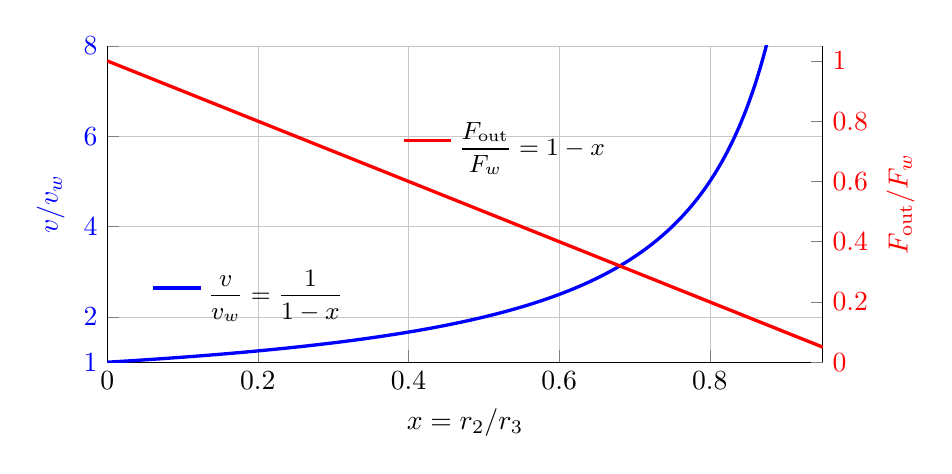
\begin{tikzpicture}
\begin{axis}[
    width=0.88\linewidth,
    height=5.6cm,
    xmin=0, xmax=0.95,
    ymin=1, ymax=8,
    xlabel={$x=r_2/r_3$},
    ylabel={$v/v_w$},
    axis y line*=left,
    axis x line*=bottom,
    ylabel style={text=blue},
    yticklabel style={text=blue},
    xtick={0,0.2,0.4,0.6,0.8},
    ytick={1,2,4,6,8},
    grid=both,
    grid style={line width=.1pt, draw=gray!25},
    major grid style={line width=.2pt, draw=gray!45},
    legend style={draw=none, fill=none, font=\small, at={(0.05,0.14)}, anchor=south west}
]
\addplot[blue, very thick, domain=0:0.95, samples=300] {1/(1-x)};
\addlegendentry{$\displaystyle \frac{v}{v_w}=\frac{1}{1-x}$}
\end{axis}

\begin{axis}[
    width=0.88\linewidth,
    height=5.6cm,
    xmin=0, xmax=0.95,
    ymin=0, ymax=1.05,
    axis y line*=right,
    axis x line=none,
    xtick=\empty,
    ylabel={$F_{\rm out}/F_w$},
    ylabel style={text=red},
    yticklabel style={text=red},
    ytick={0,0.2,0.4,0.6,0.8,1.0},
    legend style={draw=none, fill=none, font=\small, at={(0.4,0.7)}, anchor=west}
]
\addplot[red, very thick, domain=0:0.95, samples=2] {1-x};
\addlegendentry{$\displaystyle \frac{F_{\rm out}}{F_w}=1-x$}
\end{axis}
\end{tikzpicture}

\vspace{1mm}
\textbf{(a)} Gearbox tradeoff
\end{minipage}
\hfill
\begin{minipage}{0.48\textwidth}
\centering
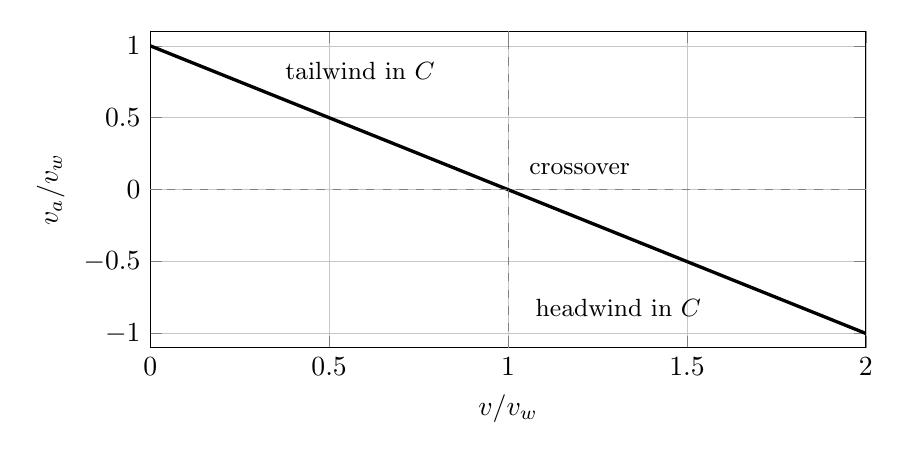
\begin{tikzpicture}
\begin{axis}[
    width=0.88\linewidth,
    height=5.6cm,
    xmin=0, xmax=2,
    ymin=-1.1, ymax=1.1,
    xlabel={$v/v_w$},
    ylabel={$v_a/v_w$},
    xtick={0,0.5,1,1.5,2},
    ytick={-1,-0.5,0,0.5,1},
    grid=both,
    grid style={line width=.1pt, draw=gray!25},
    major grid style={line width=.2pt, draw=gray!45},
]
\addplot[black, very thick, domain=0:2, samples=2] {1-x};
\addplot[dashed, gray] coordinates {(1,-1.1) (1,1.1)};
\addplot[dashed, gray] coordinates {(0,0) (2,0)};

\node[font=\small, anchor=south west] at (axis cs:0.35,0.7) {tailwind in $C$};
\node[font=\small, anchor=south west] at (axis cs:1.05,-0.95) {headwind in $C$};
\node[font=\small, anchor=south] at (axis cs:1.2,0.04) {crossover};
\end{axis}
\end{tikzpicture}

\vspace{1mm}
\textbf{(b)} Apparent wind in the vehicle frame
\end{minipage}

\caption{Dimensionless relations. (a) For \(x=r_2/r_3\), the gearbox speed ratio \(v/v_w=1/(1-x)\) grows while the useful output-force ratio \(F_{\rm out}/F_w=1-x\) falls. The output force is the net drive available at the casing, not the ground reaction. The blue curve continues above the displayed speed range. (b) The apparent-wind relation \(v_a/v_w=1-v/v_w\) changes sign at the crossover.}
\label{fig:dimensionless_plots}
\end{figure*}


Let \(F_w\) be the signed horizontal force on the gearbox from the upper rack and \(F_g\) the signed ground-rack force. Neglect gear rotational inertia, or assume steady gear rotation. Torque balance on the free upper gear equates the mesh-force magnitude to \(F_w\); torque balance on the rigid pinion--lower-gear pair then gives
\begin{equation}
F_g=-\frac{r_2}{r_3}F_w.
\label{eq:downwind-ground-force}
\end{equation}
The net drive available at the casing is
\begin{equation}
F_{\rm out}:=F_w+F_g=\frac{r_3-r_2}{r_3}F_w.
\label{eq:downwind-output-force}
\end{equation}
Under a steady opposing casing load, the load force is \(-F_{\rm out}\). Together with Eq.~\eqref{eq:amp-v-vw-ratio}, this yields the ideal input--output power relation
\begin{equation}
F_wv_w=F_{\rm out}v.
\label{eq:gearbox-power}
\end{equation}
The ground reaction is a separate force and has zero actual contact power in \(G\). With appreciable rotational acceleration, the changing gear kinetic energy must be included in the balance. Figure~\ref{fig:dimensionless_plots}(a) illustrates the useful output force decreasing as the speed ratio increases.



At \(r_2=r_3\), the no-slip constraints are incompatible with prescribed \(v_w\neq0\). Before division, the kinematic equations give
\[
v_w=\frac{r_3-r_2}{r_2}\,v_1.
\]
Thus the singularity in Eq.~\eqref{eq:v-vw-ratio} indicates a failure of the imposed rigid constraints, not a realizable infinite speed. A contact must slip or the mechanism must deform.

For the degenerate case, place two equal rolling pins one on top of the other between a table and a cutting board, constraining their centers to translate together. The three contacts are table--lower pin, lower pin--upper pin, and upper pin--board. With no slip at all three contacts, the board must remain stationary relative to the table, although the pair of pins can translate and counter-rotate. This elementary demonstration exhibits the remaining free motion when the racks have zero relative velocity.


\subsubsection{Negative Transmission (Upwind)}


The appropriate upwind analogue is the top--bottom inverted gearbox of Fig.~\ref{fig:gearboxes}(b): the gear \(r_3\), rigidly attached to pinion \(r_2\), contacts the upper rack, and free gear \(r_1\) contacts the ground. The rack velocities remain \(v_w\) and zero in \(G\). Merely inserting an idler into the original train produces a downwind branch because it changes the closure of the two rack constraints. With the same angular-velocity signs, let \(\omega_3\) describe the upper shaft and \(\omega_1\) the lower free gear.


At the upper rack--gear contact, a positive \(\omega_3\) gives a leftward
tangential velocity at the top of the gear.  Therefore the absolute velocity
of the upper contact point is
\[
v-r_3\omega_3 .
\]
No slip at the upper rack requires this to equal the rack velocity \(v_w\):
\begin{equation}
v_w = v-r_3\omega_3 .
\label{eq:upwind-upper-noslip}
\end{equation}


At the external pinion--gear mesh, equality of tooth velocities gives opposite signs for the angular velocities:

\begin{equation}
r_2\omega_3 = -\,r_1\omega_1 .
\label{eq:upwind-mesh}
\end{equation}

At the lower gear--ground contact, the lower rack is stationary in the ground
frame.  The center of the lower gear moves with velocity \(v\), while the
tangential velocity at the lower contact is \(r_1\omega_1\).  The no-slip
condition is therefore
\begin{equation}
0 = v+r_1\omega_1 .
\label{eq:upwind-lower-noslip}
\end{equation}

Equations~\eqref{eq:upwind-mesh} and~\eqref{eq:upwind-lower-noslip} imply
\[
r_1\omega_1=-v,
\qquad
r_2\omega_3=v,
\]
and hence
\[
\omega_3=\frac{v}{r_2}.
\]
Substitution into the upper no-slip condition
\eqref{eq:upwind-upper-noslip} gives
\[
v_w
 =
v-r_3\frac{v}{r_2}
 =
v\left(1-\frac{r_3}{r_2}\right)
 =
v\,\frac{r_2-r_3}{r_2}.
\]
Solving for \(v/v_w\), one obtains
\begin{equation}
\frac{v}{v_w}
=
-\frac{r_2}{r_3-r_2}
\qquad\text{(negative transmission).}
\label{eq:upwind-v-vw-ratio}
\end{equation}

For \(r_3>r_2\) and \(v_w>0\), the casing moves upwind. For the same radii in the two orientations, define
\[
D_{\rm down}:=\frac{v_{\rm down}}{v_w}=\frac{r_3}{r_3-r_2},
\qquad
D_{\rm up}:=\frac{v_{\rm up}}{v_w}=-\frac{r_2}{r_3-r_2}.
\]
They obey
\begin{equation}
D_{\rm down}+D_{\rm up}=1,
\qquad D_{\rm up}=1-D_{\rm down}.
\label{eq:upwind-downwind-symmetry}
\end{equation}
Upwind motion requires \(r_3>r_2\); faster-than-the-wind upwind motion further requires
\[
|D_{\rm up}|=\frac{r_2}{r_3-r_2}>1.
\]
Together these conditions give
\begin{equation}
r_2<r_3<2r_2.
\label{eq:upwind-amplification-condition}
\end{equation}
Equivalently, the associated downwind orientation has \(D_{\rm down}>2\). These identities are kinematic properties of the inverted rack model.



Under the same negligible-rotational-inertia or steady-rotation assumption, torque balance now gives
\begin{align}
F_g&=-\frac{r_3}{r_2}F_w,
\label{eq:upwind-ground-force}\\
F_{\rm out}&=F_w+F_g=-\frac{r_3-r_2}{r_2}F_w.
\label{eq:upwind-output-force}
\end{align}
Thus \(F_{\rm out}\) and \(v\) are both negative when \(F_w\) and \(v_w\) are positive, and Eq.~\eqref{eq:gearbox-power} still holds. The useful output-force magnitude satisfies
\begin{equation}
|F_{\rm out}|=\frac{r_3-r_2}{r_2}|F_w|.
\label{eq:upwind-force-ratio}
\end{equation}
Again, this is the force available at the casing, not the larger ground reaction. Speed amplification reduces useful output force. The physical upwind cart realizes the corresponding transfer with a turbine driving its wheels.



\begin{figure*}[htbp]
\centering
\begin{tabular}{@{}c@{\hspace{6mm}}c@{}}
\begin{tikzpicture}[
    scale=0.95, transform shape,
    line cap=round,
    line join=round,
    >=Stealth,
    font=\normalsize
  ]
  \useasboundingbox (-4.2,0.6) rectangle (4.5,7.2);

  \begin{scope}[yshift=1.5cm]

    % Key points
    \coordinate (P)   at (0,0);      % pivot
    \coordinate (T)   at (0,4.6);    % top of lever (current)
    \coordinate (Tf)  at (62:4.6); % top of lever (rotated / future)

    % Ground
    \draw[thick] (-4.0,0) -- (4.1,0);

    % Pivot support
    \draw[thick] (-0.18,-0.22) -- (P) -- (0.18,-0.22) -- cycle;
    \fill (0,0) circle (2pt);

    % Current lever / mast
    \draw[thick] (P) -- (T);

    % Current platform
    \draw[thick] (-0.55,4.6) -- (0.55,4.6);

    % Future/rotated position (draw first, so sail box can cover it)
    \draw[dashed,draw=black] (P) -- (Tf);
    \draw[dashed,draw=black] ($(Tf)+(152:0.55)$) -- ($(Tf)+(-28:0.55)$);

    % Sail box, opaque
    \draw[thick, fill=white] (-1.05,0.95) rectangle (1.05,2.35);
    \node at (0,1.65) {sail};

    % Rotation arrow as a circular arc centered at the pivot P
    \draw[->,line width=1pt] ($(P)+(87:3.5)$) arc[start angle=87,end angle=65,radius=3.5];

    % Wind arrows
    \node at (-3.0,4.2) {wind};
    \foreach \y in {3.0,2.1,1.2}{
      \draw[->,thick,decorate,decoration={snake,amplitude=2pt,segment length=18pt}]
        (-3.75,\y) -- (-1.95,\y);
    }

    % Platform label
    \node at ($(P)+(0,5.0)$) {platform};
    \node at ($(P)+(0,-0.55)$) {pivot};

  \end{scope}
\end{tikzpicture}
&
\begin{tikzpicture}[
    scale=0.95, transform shape,
    line cap=round,
    line join=round,
    >=Stealth,
    font=\normalsize
  ]
  \useasboundingbox (-4.2,-0.4) rectangle (4.5,8.2);

  % Angles
  \def\thCur{15}   % current lever angle
  \def\thFut{58}   % future lever angle

  % Wind arrows and label (kept fixed)
  \node at (-0.55,4.55) {wind};
  \draw[->,thick,decorate,decoration={snake,amplitude=2pt,segment length=18pt}]
    (-4.0,4.15) -- (-2.85,3.25);
  \draw[->,thick,decorate,decoration={snake,amplitude=2pt,segment length=18pt}]
    (-3.55,4.75) -- (-2.35,3.85);
  \draw[->,thick,decorate,decoration={snake,amplitude=2pt,segment length=18pt}]
    (-3.1,5.15) -- (-1.9,4.25);

  % Entire lever arrangement shifted upward by 1 units
  \begin{scope}[yshift=1cm]

    % Key points
    \coordinate (P)       at (1.05,1.25);                    % pivot
    \coordinate (Sattach) at ($(P)+({180+\thCur}:2.45)$);   % sail attachment point on lever
    \coordinate (R)       at ($(P)+(\thCur:2.95)$);         % current right end
    \coordinate (Rf)      at ($(P)+(\thFut:2.95)$);         % future right end / platform center
    \coordinate (Rb)      at ($(P)+({180+\thFut}:2.45)$);   % lower dashed extension

    % Current lever: exactly through pivot
    \draw[thick] (Sattach) -- (R);

    % Future/rotated lever position (dashed): extended below, cut at tilted platform
    \draw[dashed,draw=black] (Rb) -- (Rf);

    % Pivot support: same size/style as previous drawing
    \draw[thick] ($(P)+(-0.18,-0.22)$) -- (P) -- ($(P)+(0.18,-0.22)$) -- cycle;
    \fill (P) circle (2pt);

    % Current platform: perpendicular to current lever
    \draw[thick] ($(R)+({\thCur+90}:0.55)$) -- ($(R)+({\thCur-90}:0.55)$);

    % Future platform: perpendicular to future lever, dashed
    \draw[dashed,draw=black] ($(Rf)+({\thFut+90}:0.55)$) -- ($(Rf)+({\thFut-90}:0.55)$);

    % Sail box: smaller, moved closer to the pivot
    \node[
      draw,
      thick,
      fill=white,
      minimum width=1.20cm,
      minimum height=2.10cm,
      rotate=\thCur,
      anchor=east,
      inner sep=0pt
    ] at (Sattach) {sail};

    % Rotation arrows as circular arcs centered at the pivot P
    \draw[->,line width=1pt] ($(P)+(200:1.15)$) arc[start angle=200,end angle=234,radius=1.15];
        \draw[->,line width=1pt] ($(P)+(18:2.0)$)   arc[start angle=18,end angle=56,radius=2.0];

    % Labels
    \node at ($(Rf)+(1.0,0.10)$) {platform};
    \node at ($(P)+(0.20,-0.55)$) {pivot};

  \end{scope}
\end{tikzpicture}
\\
(a) Downwind Analogy & (b) Upwind Analogy
\end{tabular}
\caption{Lever geometry at representative instants. (a) A fixed pivot at one end gives a tip speed greater than the sail-point speed by \(L/d_s\). (b) Placing the pivot between the sail and tip reverses their instantaneous velocity directions. Exceeding the wind speed also depends on the sail-point velocity and lever-arm ratio; the finite stroke permits only transient motion.}
\label{fig:lever-downupwind}
\end{figure*}

\subsection{The Lever Analogy}


A lever illustrates the force--speed tradeoff through geometry. Its fixed pivot permits rotation and supplies reaction forces, but an ideal frictionless pivot applies no reaction couple about its own axis. A lever has a finite stroke; the cart's rotary drivetrain permits continuous operation.

\subsubsection{With the Wind}

Consider a rigid lever of length \(L\), with a sail at distance \(d_s\) from the fixed pivot [Fig.~\ref{fig:lever-downupwind}(a)]. At the illustrated instant the lever is perpendicular to the wind, so the tangential velocities are parallel to it. Let the sail-point speed be \(v_s=\alpha v_w\), with \(0<\alpha<1\) an assumed instantaneous velocity fraction, not a power efficiency. Then

\begin{equation}
\omega = \frac{v_s}{d_s}.
\end{equation}
The velocity of the distal end is then
\begin{equation}
v_d = \omega L = \alpha \left(\frac{L}{d_s}\right) v_w.
\end{equation}

The geometric tip-to-sail speed ratio is \(L/d_s\). The tip exceeds \(v_w\) when \(L/d_s>1/\alpha\). For tangential input and output forces, negligible angular acceleration gives the corresponding force relation

\begin{equation}
F_d = F_w \frac{d_s}{L},\label{eq:lever-force}
\end{equation}

Here \(F_d\) is the magnitude of the resisting output load at the tip. If rotational inertia is retained, the torque balance is \(F_wd_s-F_dL=I\dot\omega\), rather than Eq.~\eqref{eq:lever-force}. The pivot reaction can have a moment about other reference points, but its moment about the pivot itself is zero.


\subsubsection{Against the Wind}


With the pivot between the sail and tip [Fig.~\ref{fig:lever-downupwind}(b)], their instantaneous tangential velocities point in opposite directions. Let \(d_p\) be the sail-to-pivot distance and \(L-d_p\) the pivot-to-tip distance. For the component comparison along the wind, use an instant when the lever is perpendicular to it; the tilted drawing illustrates rotation more generally. With \(v_s=\alpha v_w\),

\begin{equation}
\omega = \frac{v_s}{d_p}.
\end{equation}
The velocity at the opposite end is
\begin{equation}
v_d = -\omega (L - d_p) = -\alpha \left(\frac{L - d_p}{d_p}\right) v_w.
\end{equation}

The negative sign denotes the reversal. The tip speed magnitude exceeds \(v_w\) when \((L-d_p)/d_p>1/\alpha\). These instantaneous geometric relations illustrate amplification and reversal without implying sustained translation of the whole lever.


\subsection{The Popescu Glide: No Propulsion from Internal Forces Alone}


Internal forces alone cannot change the center-of-mass motion of a closed system. Consider the ``Popescu Glide'' thought experiment~\cite{popescu_talk_2024}: Alice stands on a dock and Bob walks toward her inside a boat initially at rest, with negligible horizontal water resistance [Fig.~\ref{fig:popescu-glide}]. The boat recoils, and the mass-weighted displacements of Bob and boat cancel. Bob's own displacement need not vanish.


Let Bob have mass $m$ and the boat mass $M$. If Bob walks a distance $l$ relative to the boat, the boat must move backward by a distance $\Delta x_\text{boat}$ such that the system's center of mass does not shift:
\begin{equation}
m\,\Delta x_\text{Bob} + M\,\Delta x_\text{boat} = 0.
\end{equation}
Since Bob's displacement relative to the water is the sum of his motion relative to the boat and the boat's recoil,
\begin{equation}
\Delta x_\text{Bob} = l + \Delta x_\text{boat},
\end{equation}
we obtain
\begin{equation}
m(l + \Delta x_\text{boat}) + M\,\Delta x_\text{boat} = 0.
\end{equation}
Solving for the boat's recoil gives
\begin{equation}
\Delta x_\text{boat} = -\frac{m}{m+M}\,l.
\end{equation}
The negative sign indicates the boat moves backward. Bob's resulting progress toward Alice, measured relative to the water, is therefore
\begin{equation}
\Delta x_\text{Bob} = l - \frac{m}{m+M}\,l = \frac{M}{m+M}\,l.
\end{equation}

Bob therefore gets closer to Alice even in the ideal model, by the fraction \(M/(m+M)\) of his walking distance. Whether he reaches the dock depends on its initial separation and the available distance \(l\). The limit \(M\to\infty\) suppresses recoil through inertia alone; it does not require attaching the boat to an external support.

The limitation concerns the \emph{combined center of mass}. Returning Bob to his original position within the boat restores the original boat position in this idealization, so cyclic internal rearrangement cannot provide repeated propulsion. A wind cart is instead an open mechanical system: its rotor exchanges momentum with air and its wheels with ground. Wind acting on a rotor is already an external interaction and must not be treated as an internal force in a closed-system argument.


\begin{figure}[htbp]
\centering
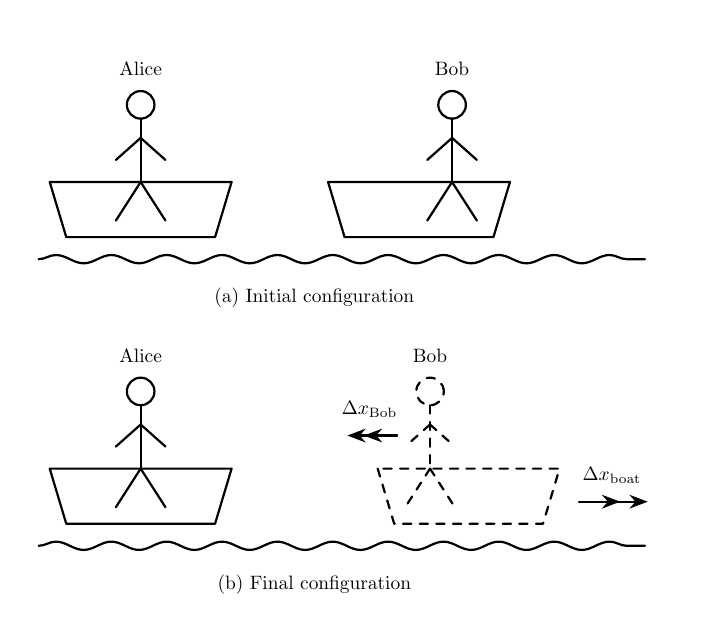
\begin{tikzpicture}[
    scale=0.7, transform shape,
    line cap=round,
    line join=round,
    >=Stealth,
    font=\normalsize
  ]
  \useasboundingbox (-5.2,-0.8) rectangle (6.6,9.4);

  %============================
  % TOP PANEL: INITIAL
  %============================
  \begin{scope}[yshift=5.2cm]

    \node[above] at (0,-1) {(a) Initial configuration};

    % Water surface (wavy)
    \draw[thick,decorate,decoration={snake,amplitude=1.5pt,segment length=20pt}]
      (-5.0,0) -- (6.0,0);

    % Left side: Alice
    \begin{scope}[shift={(-3.0,0.4)}]
      % Boat / dock outline
      \draw[thick, fill=white] (-1.8,1.0) -- (-1.5,0) -- (1.2,0) -- (1.5,1.0) -- cycle;

      % Alice (stick figure)
      \draw[thick] (-0.15,2.4) circle (0.25);     % head
      \draw[thick] (-0.15,2.15) -- (-0.15,1.0);   % body
      \draw[thick] (-0.15,1.8) -- (-0.6,1.4);     % left arm
      \draw[thick] (-0.15,1.8) -- (0.3,1.4);      % right arm
      \draw[thick] (-0.15,1.0) -- (-0.6,0.3);     % left leg
      \draw[thick] (-0.15,1.0) -- (0.3,0.3);      % right leg

      \node[above] at (-0.15,2.8) {Alice};
    \end{scope}

    % Right side: Bob's boat, initial state only
    \begin{scope}[shift={(1.55,0.4)}]
      % Initial boat (solid)
      \draw[thick, fill=white] (-1.3,1.0) -- (-1.0,0) -- (1.7,0) -- (2.0,1.0) -- cycle;

      % Initial Bob (solid): on the right side of the boat
      \draw[thick] (0.95,2.4) circle (0.25);      % head
      \draw[thick] (0.95,2.15) -- (0.95,1.0);     % body
      \draw[thick] (0.95,1.8) -- (0.50,1.4);      % left arm
      \draw[thick] (0.95,1.8) -- (1.40,1.4);      % right arm
      \draw[thick] (0.95,1.0) -- (0.50,0.3);      % left leg
      \draw[thick] (0.95,1.0) -- (1.40,0.3);      % right leg

      \node[above] at (0.95,2.8) {Bob};
    \end{scope}

  \end{scope}

  %============================
  % BOTTOM PANEL: FINAL
  %============================
  \begin{scope}[yshift=0cm]

   \node[above] at (0,-1) {(b) Final configuration};

    % Water surface (wavy)
    \draw[thick,decorate,decoration={snake,amplitude=1.5pt,segment length=20pt}]
      (-5.0,0) -- (6.0,0);

    % Left side: Alice
    \begin{scope}[shift={(-3.0,0.4)}]
      % Boat / dock outline
      \draw[thick, fill=white] (-1.8,1.0) -- (-1.5,0) -- (1.2,0) -- (1.5,1.0) -- cycle;

      % Alice (stick figure)
      \draw[thick] (-0.15,2.4) circle (0.25);     % head
      \draw[thick] (-0.15,2.15) -- (-0.15,1.0);   % body
      \draw[thick] (-0.15,1.8) -- (-0.6,1.4);     % left arm
      \draw[thick] (-0.15,1.8) -- (0.3,1.4);      % right arm
      \draw[thick] (-0.15,1.0) -- (-0.6,0.3);     % left leg
      \draw[thick] (-0.15,1.0) -- (0.3,0.3);      % right leg

      \node[above] at (-0.15,2.8) {Alice};
    \end{scope}

    % Right side: Bob's boat, final state only (dashed)
    \begin{scope}[shift={(2.45,0.4)}]
      % Final boat (dashed)
      \draw[dashed, thick] (-1.3,1.0) -- (-1.0,0) -- (1.7,0) -- (2.0,1.0) -- cycle;

      % Final Bob (dashed): shifted left relative to the boat
      \draw[dashed, thick] (-0.35,2.4) circle (0.25);     % head
      \draw[dashed, thick] (-0.35,2.15) -- (-0.35,1.0);   % body
      \draw[dashed, thick] (-0.35,1.8) -- (-0.80,1.4);    % left arm
      \draw[dashed, thick] (-0.35,1.8) -- (0.10,1.4);     % right arm
      \draw[dashed, thick] (-0.35,1.0) -- (-0.80,0.3);    % left leg
      \draw[dashed, thick] (-0.35,1.0) -- (0.10,0.3);     % right leg

      \node[above] at (-0.35,2.8) {Bob};
    \end{scope}

    % Displacement arrows and labels
    % Bob's motion relative to the water: leftward
    \draw[->,thick] (1.5,2) -- (0.9,2);
    \draw[->,thick] (1.5,2) -- (0.6,2);
    \node[above] at (1,2.2) {$\Delta x_{\mathrm{Bob}}$};

    % Boat recoil: rightward
    \draw[->,thick] (4.9,0.8) -- (5.55,0.8);
    \draw[->,thick] (4.8,0.8) -- (6.05,0.8);
    \node[above] at (5.4,1) {$\Delta x_{\mathrm{boat}}$};

  \end{scope}

\end{tikzpicture}
\caption{The ``Popescu Glide.'' (a) Initial state. (b) Bob walks leftward while the boat recoils rightward. Bob gets closer to Alice, but the mass-weighted displacements cancel and the combined center of mass remains fixed in the ideal model with negligible horizontal external force.}
\label{fig:popescu-glide}
\end{figure}


McDonald noted two further ways in which the idealization can fail to capture Bob's access to the dock~\cite{McDonald2026priv}. First, Bob can jump and land on a sufficiently close dock. Momentum is conserved during push-off, but the subsequent dock contact supplies an external impulse. Second, water drag opposes the boat's backward recoil when Bob walks forward, transferring momentum to the water and altering the combined center-of-mass motion. That drag dissipates energy; quiescent water supplies no net energy in this process.

The analogy therefore isolates the difference between internal rearrangement and external momentum exchange. A fixed support is one possible source of reaction, rather than a universal requirement for every kind of propulsion.


\section{Pedagogical Use: Teaching Levels, Learning Goals, Misconceptions, and Activities}
\label{sec:pedagogy}

The phenomenon and its analogies lend themselves to rich instruction from secondary school through undergraduate mechanics and laboratory courses. This section provides a concise, ready-to-use guide.

\subsection{Target levels and prerequisites}

\begin{itemize}
\item Secondary/high school (ages 15--18): Newton's laws, reference frames, work--energy, static versus kinetic friction, and basic gears or levers.
\item Introductory undergraduate physics/engineering: Rates of mechanical energy transfer, efficiency, drag scaling, turbines vs fans, idealizations vs nonidealities.
\item Upper-level mechanics/fluids: Constraint forces and power flow, momentum exchange between media, efficiency and performance limits, modeling/simulation.
\end{itemize}

\subsection{Learning goals}

By the end of instruction, students should be able to:
\begin{enumerate}
\item Distinguish airspeed, ground speed, and apparent wind; compute frame-dependent velocities.
\item Explain how static friction can transmit force without doing work in the ground frame; identify where mechanical energy enters and leaves the system and the corresponding rates of transfer.
\item Describe the vehicle as a mechanical transformer between two media; draw qualitative rate-of-energy-transfer (power-flow) diagrams for downwind and upwind operation.
\item Use the gearbox/lever analogies to predict velocity amplification and force reduction; derive and interpret the velocity-amplification factor $v/v_w = r_3/(r_3-r_2)$ in Eq.~\eqref{eq:amp-v-vw-ratio}.
\item Explain how the wind vehicles considered here couple environments in relative motion, and distinguish their external momentum exchange from the closed-system boat example.
\item Predict qualitative effects of changing gear ratio or blade pitch on achievable speed ratio and thrust.
\item Diagnose and correct common misconceptions (Section~\ref{sec:misconceptions}).
\end{enumerate}

\subsection{Typical conceptions and misconceptions}
\label{sec:misconceptions}

\begin{itemize}
\item ``If the cart matches the wind speed, the apparent wind is zero, so it can't accelerate further.''
\\Resolution: Driven rotation induces flow even at zero far-field apparent wind. Equations~\eqref{eq:cart-shaft-power}--\eqref{eq:cart-net-drive} show the finite shaft power and the condition for positive net drive. The air can lose energy in \(G\) while the fan adds energy to the flow in \(C\).

\item ``The ground must do positive work on the cart to speed it up.''
\\Resolution: Ideal no-slip contact has zero instantaneous velocity in \(G\), hence zero contact power. Its force and torque redistribute energy between translation and rotation; wind supplies the net energy.

\item ``This violates energy conservation.''
\\Resolution: No violation occurs. The mechanism couples two media and is not a single-turbine extraction from a uniform airstream.

\item ``A plane can't do this, so a cart can't either.''
\\Resolution: In uniform wind, a free aircraft lacks the cart's air--ground coupling. Wind shear and auxiliary power are different cases, outside that argument.

\item Frame confusion: mixing air-frame and ground-frame velocities and rates of energy transfer.
\\Resolution: Require explicit statements of the chosen frame and draw power-flow arrows with signs and reference frames.
\end{itemize}

\subsection{Classroom activities and exercises}

\begin{itemize}
\item Lever analogy (Fig.~\ref{fig:lever-downupwind}): Mount a meter stick on a fixed pivot that allows rotation. Compare instantaneous speeds at two distances from the pivot, then place the pivot between the points to reverse their velocity directions. Distinguish pivot reaction forces from a couple about its own axis.
\item Popescu Glide: On a low-friction cart with enough room to move, a student shifts toward one end. Observe both the student's progress and the cart's recoil; compare their mass-weighted displacements. A wall-mounted rope provides an external interaction that changes the center-of-mass motion.
\end{itemize}

\subsection{Conceptual and quantitative exercises}

\begin{enumerate}
\item Conceptual (frames): In the ground frame, explain how the ground does no work on the cart in the ideal rolling limit, yet the cart accelerates. Where does the power come from?

\item Power balance at the crossover: Set \(v=v_w\) in Eqs.~\eqref{eq:cart-shaft-power}--\eqref{eq:cart-air-power}. Identify the induced flow, shaft-power demand, wheel reaction, and condition for acceleration. Explain the different fluid-energy signs in \(C\) and \(G\).

\item Upwind variant: Using the top--bottom inverted negative-transmission gearbox, explain why the cart can move upwind. How does the sign of $v/v_w$ change, and why is the upwind magnitude not generally the same as the downwind magnitude?
\end{enumerate}

\subsection{Assessment ideas and rubrics (brief)}

\begin{itemize}
\item Exit ticket: ``In one or two sentences, explain why the ground can provide a force yet do no work on the cart.''
\item Short quiz: Multiple-choice on frames and signs of power; one free-response drawing a rate-of-energy-transfer (power-flow) diagram.
\item Lab report: Methods (measurement of $v_w$ and $v$), uncertainty estimates, and a discussion relating data to the gearbox/lever analogies.
\end{itemize}


\section{Conclusion}


Faster-than-the-wind travel follows from coupling environments in relative motion through a drivetrain. The explicit downwind balance separates shaft power from ground-frame fluid energy: a driven fan can produce thrust while the cart gains energy and the air loses it. Traction enables momentum exchange at the ground, whose ideal instantaneous contact power is zero.

The gearbox makes the force--speed tradeoff exact within a rigid-rack model; its useful output force must be distinguished from the ground reaction. The lever illustrates instantaneous amplification and reversal over a finite stroke. The boat example shows that internal rearrangement can bring one component closer to a destination while leaving the closed system's center of mass unchanged.

These mechanisms retain an Archimedean lesson: a lever or tackle trades force for displacement and requires a suitable reaction support~\cite[pp.~14--17]{dijksterhuis_archimedes_2014}. On the cart, ground traction supplies that reaction; on water, momentum transfer to the fluid entails wake losses. Neither coupling alone nor a large ideal ratio guarantees motion above the wind speed: adequate net drive and sufficiently small losses are required. The examples offer complementary ways to teach constraints, reference frames, momentum exchange, and mechanical power.


\begin{acknowledgments}
The author thanks Sandu Popescu for a helpful communication regarding his inspiring boat analogy, and Kirk Thomas McDonald for stimulating and constructive criticism of earlier versions of the manuscript. Any remaining errors or misconceptions are the author's responsibility.
This research was funded in whole or in part by the \textit{Austrian Science Fund (FWF)} [Grant \href{https://doi.org/10.55776/PIN5424624}{DOI:10.55776/PIN5424624}].
The author acknowledges TU Wien Bibliothek for financial support through its Open Access Funding Programme.

This text was partially created and revised with assistance from large language models. All content, ideas, and prompts were provided by the author.
\end{acknowledgments}

\bibliography{svozil}

\end{document}
